\documentclass[12pt]{article}\usepackage[]{graphicx}\usepackage[]{color}
% maxwidth is the original width if it is less than linewidth
% otherwise use linewidth (to make sure the graphics do not exceed the margin)

\usepackage{scrtime} % for \thistime (this package MUST be listed first!)
\usepackage[margin=1in]{geometry}
\usepackage[usenames,dvipsnames]{xcolor}
\definecolor{aqua}{RGB}{0, 128, 225}
\usepackage[colorlinks=true,citecolor=aqua,linkcolor=aqua,urlcolor=aqua,hypertexnames=false]{hyperref}
\usepackage{xspace}
\usepackage{tikz}
\usepackage{placeins} % \FloatBarrier
\usepackage{amsmath} % \text, \cases
\usepackage{enumerate} % fancier enumeration (e.g., a,b,c, ...)
\usepackage{ragged2e} % \RaggedRight
\usepackage{grffile} % \RaggedRight

%% cleveref package for convenient hyperrefercing/citing:
\usepackage[nameinlink,capitalize]{cleveref}
\crefname{equation}{Equation}{Equations}
\Crefname{equation}{Equation}{Equations}
\crefname{figure}{Figure}{Figures}
\Crefname{figure}{Figure}{Figures}
\crefname{section}{\S}{\SS}
\Crefname{section}{\S}{\SS}

%% line numbers
\usepackage{lineno}\renewcommand\thelinenumber{\color{gray}\arabic{linenumber}}

%% comments
\newcommand{\hidecomments}{\renewcommand{\comment}[3]{}}
\newcommand{\comment}[3]{\textcolor{#1}{\textbf{[#2: }\textit{#3}\textbf{]}}}
\newcommand{\david}[1]{\comment{magenta}{DE}{#1}}
\newcommand{\jd}[1]{\comment{blue}{JD}{#1}}
\newcommand{\ben}[1]{\comment{purple}{BB}{#1}}
\newcommand{\mike}[1]{\comment{orange}{ML}{#1}}

%% code
\newcommand{\code}[1]{{\tt #1}}

%% misc macros
\newcommand{\etal}{\textit{et al}.\xspace}
%% for referencing TeX macros:
\newcommand\ttbackslash{{\tt\char`\\}}
\newcommand{\macro}[1]{{\tt\ttbackslash#1}}
\newcommand{\term}[1]{{\bfseries\slshape#1}}
\newcommand{\thickredline}{{\color{red}\bigskip\begin{center}\linethickness{2mm}\line(1,0){250}\end{center}\bigskip}}

%% abbreviations
\newcommand{\ie}{\emph{i.e., }}
\newcommand{\eg}{\emph{e.g., }}
\newcommand{\etc}{\emph{etc.}\xspace}

%% notation
\newcommand{\emx}[1]{\ensuremath{#1}\xspace}
\newcommand{\R}{\emx{{\mathcal R}}}
\newcommand{\Rzero}{{\mathcal R}_0}
\newcommand{\Rt}{\emx{{\mathcal R}_t}}
\newcommand{\littler}{\emx{r}}
\newcommand{\littlerwt}{\emx{r_{WT}}}
\newcommand{\littlervoc}{\emx{r_{VOC}}}
\newcommand{\B}{\emx{\beta}}
\newcommand{\Bwt}{\emx{\beta_{WT}}}
\newcommand{\Bvoc}{\emx{\beta_{VOC}}}
\newcommand{\textsub}[2]{\emx{{#1}_{\textrm{\small #2}}}}
\newcommand{\pmob}{\textsub{p}{mob}}


%% settings
\date{\today\ @ \thistime}

\definecolor{fgcolor}{rgb}{0.345, 0.345, 0.345}
\newcommand{\hlnum}[1]{\textcolor[rgb]{0.686,0.059,0.569}{#1}}%
\newcommand{\hlstr}[1]{\textcolor[rgb]{0.192,0.494,0.8}{#1}}%
\newcommand{\hlcom}[1]{\textcolor[rgb]{0.678,0.584,0.686}{\textit{#1}}}%
\newcommand{\hlopt}[1]{\textcolor[rgb]{0,0,0}{#1}}%
\newcommand{\hlstd}[1]{\textcolor[rgb]{0.345,0.345,0.345}{#1}}%
\newcommand{\hlkwa}[1]{\textcolor[rgb]{0.161,0.373,0.58}{\textbf{#1}}}%
\newcommand{\hlkwb}[1]{\textcolor[rgb]{0.69,0.353,0.396}{#1}}%
\newcommand{\hlkwc}[1]{\textcolor[rgb]{0.333,0.667,0.333}{#1}}%
\newcommand{\hlkwd}[1]{\textcolor[rgb]{0.737,0.353,0.396}{\textbf{#1}}}%
\let\hlipl\hlkwb

\usepackage{framed}
\makeatletter
\newenvironment{kframe}{%
 \def\at@end@of@kframe{}%
 \ifinner\ifhmode%
  \def\at@end@of@kframe{\end{minipage}}%
  \begin{minipage}{\columnwidth}%
 \fi\fi%
 \def\FrameCommand##1{\hskip\@totalleftmargin \hskip-\fboxsep
 \colorbox{shadecolor}{##1}\hskip-\fboxsep
     % There is no \\@totalrightmargin, so:
     \hskip-\linewidth \hskip-\@totalleftmargin \hskip\columnwidth}%
 \MakeFramed {\advance\hsize-\width
   \@totalleftmargin\z@ \linewidth\hsize
   \@setminipage}}%
 {\par\unskip\endMakeFramed%
 \at@end@of@kframe}
\makeatother

\makeatletter
\def\maxwidth{ %
  \ifdim\Gin@nat@width>\linewidth
    \linewidth
  \else
    \Gin@nat@width
  \fi
}
\makeatother



\title{A compartmental model for epidemic parameter estimation and forecasting, with applications to COVID-19 variant-of-concern spread}

\author{Michael Li, Jonathan Dushoff, David Earn, Irena Papst, Nick Ogden and Benjamin M. Bolker\\
  McMaster University\\
  \url{https://mac-theobio.github.io/covid-19/}
  }


\begin{document}

\linenumbers
\maketitle

\section*{Story:}
\begin{enumerate}
\item{Basic macpan}
\item{time-varying parameters to model the effect of shutdowns and reopening}
\item{ad-hoc VOC}
\end{enumerate}

\begin{abstract}
\mike{NEED TO FIX! What is the story we are trying to tell?}
  Virological testing and contact tracing are being used by many
  jurisdictions that are attempting to mitigate the spread of
  SARS-CoV-2.  How much testing and tracing is necessary for control
  is not clear and must be explored with models.  We show how testing
  and tracing can be integrated in a compartmental epidemic model, and
  find that without contact tracing, testing and isolation of infected
  individuals is unlikely to have a significant impact on the spread
  of SARS-CoV-2.  We use maximum likelihood estimation to calibrate
  the model to multiple COVID-19 time series (positive tests, negative
  tests, hospitalizations, and deaths) for each of the Canadian
  provinces from 2020-02-27 to 2020-08-30.  We
  estimate epidemiological parameters, including the effective
  reproduction number $\R_t$ over the course of the epidemic.
  %% 
  \david{mention mobility data? epidemiologically salient parameters
    that we estimate? \dots}
  \ben{tempted to wordsmith like crazy, should resist the urge and
    work on the body of text instead. Quick comments: (1) should say
    a little less about tracing, since that part really isn't in our
    model explicitly (implicit via the weights, we can talk about that
    a bit, but it seems like false advertising to discuss it in the abstract);
    (2) A little bit more emphasis on the fact that we have built a flexible,
    generally useful model for simulation and calibration (time-varying parameters,
    incorporation of covariates on transmission rate, etc.)}
\end{abstract}

%%\vfill
%%\subsubsection*{Our group's COVID-19 research}
%% A brief summary, including publications by our group to date, is available at\\
%%\url{https://mac-theobio.github.io/covid-19/}.
%%\david{I updated Park et al 2020, which is now published in JRSI.  JD,
%%  please update that page with anything else you've published.}

%%\vfill

\tableofcontents

%%\vfill

%%\subsubsection*{\underline{Current date range for analysis}: \ \ date_range[1] -- date_range[2]}

%%\newpage

\section{Introduction}

SARS-CoV-2, the
etiological agent of coronavirus disease 2019 (COVID-19), has been
circulating in Canada since at least January 2020 \cite{onpr_200125}.
Response to the worldwide pandemic \cite{Li+20,Fauc+20} has been
guided to a substantial extent by mathematical modelling
\cite{Flax+20}.

%% Virological testing and contact tracing have been conducted to varying
%% degrees in different jurisdictions\david{REFS}.  While testing is
%% imperative for surveillance, its value for control is less clear.
%% Agent-based simulations indicate that the combination of testing and
%% contact tracing can be very effective in mitigating spread of
%% SARS-CoV-2 \cite{Ng+20}.  Emerging research is demonstrating that
%% saliva-based tests, as opposed to naso-pharyngeal swabs for RT-qPCR,
%% may be more effective, cheaper, and viable for the public to
%% self-administer \cite{Will+20,Wyll+20}, potentially making very
%% large-scale, frequent testing possible.

Here, we present a compartmental framework that has been developed
over the course of the pandemic. It incorporates the standard epidemiological compartments
required to model COVID-19 as well as compartments that track health-care utilization and COVID-induced
mortality. Case reporting can be modeled either as a time-delayed convolution
of incidence or by enabling a factorial expansion of the model that accounts
for the testing status of individuals [CITE Friston, ?]. The model also allows
for time-dependent variation in any rate parameter --- particularly the transmission rate --- and
allows this variation to be indexed by external covariates such as cellphone-based mobility
metrics, or to follow smooth (spline) curves over time. The same model structure can be
run as an ordinary differential equation,
a discrete-time-step deterministic model, or
a discrete-time-step stochastic model with dynamical noise.
Finally, the model can be used to
(1) simulate specific scenarios for planning purposes; 
(2) calibrate parameters to match multiple input time series such as hospital admissions or occupancy, cases, or deaths; or
(3) forecast future epidemic dynamics on the basis of past calibration.

\section{Methods}

\subsubsection*{Compartmental mechanistic model}

The epidemiological structure of the model is based on
a susceptible-exposed-infectious-removed (SEIR) model with
additional compartments reflecting the biology of COVID-19 and the
structure of the health-care system. The COVID-19-specific compartmental structure
of the model resembles many other COVID-19 models
\ben{orig Stanford model is at \url{https://www.ncbi.nlm.nih.gov/pmc/articles/PMC7276010/}, preprint only? Feeling
  lazy, but we should probably dig up 2 or 3 examples}
in splitting the usual single infectious compartment into sub-compartments reflective
of the epidemiology of COVID-19; it additionally adds
compartments for hospitalized individuals in acute care
or intensive care. All symptomatic individuals are
presumed to have undergone a period of pre-symptomatic infectiousness
(\code{p}). Infections can be
asymptomatic (\code{a}), mildly or moderately symptomatic (\code{m}) or
severely symptomatic (\code{s}); all individuals with severe symptoms
go to the hospital (acute care or ICU), and all individuals who die (\code{d}) are assumed to have
have spent time in the ICU.  Recovered individuals (\code{R}) are
assumed to be immune.  The model flow chart
(\cref{fig:flowchart}) and flow matrix (\cref{fig:flowmatrix})
include additional compartments which facilitate book-keeping:
cumulative hospital admissions (\code{X}), individuals in acute care
after discharge from ICU (\code{H2}), and cumulative deaths
(\code{D}).

%%\begin{figure}[ht!]
\begin{figure}
\definecolor{shadecolor}{rgb}{0.969, 0.969, 0.969}\color{fgcolor}
\includegraphics[width=\maxwidth]{figure/flowchart.pdf}
\caption{Flow chart for basic compartmental mechanistic transmission
  model. Compartments: \code{S} (susceptible), \code{E} (exposed),
  \code{Ia} (asymptomatic infection), \code{Ip} (presymptomatic
  infection), \code{Im} (mild/moderately symptomatic infection),
  \code{Is} (severely symptomatic infection), \code{H} (hospitalized
  [acute care]), \code{ICUs} (ICU with prognosis of survival),
  \code{ICUd} (ICU with prognosis of death), \code{H2} (acute care
  after ICU stay), \code{R} (recovered), \code{D} (dead), \code{X}
  (accumulator for cumulative hospital admissions).
  \ben{possible tweaks: colour? straight arrows? restore flow symbols on arrows? adjust box widths based on chars in compartment
name? lose the shadows?}}
\label{fig:flowchart}
\end{figure}

\begin{figure}[ht!]
\definecolor{shadecolor}{rgb}{0.969, 0.969, 0.969}\color{fgcolor}
\includegraphics[width=\maxwidth]{figure/ratematrix.pdf} 

\caption{Flow matrix for basic compartmental mechanistic transmission
  model.  Gray indicates non-zero flows: compartments as in
  \cref{fig:flowchart}.  \ben{do we want this? It's equivalent to
    the flowchart, could be used to show differences in magnitude (via shading)
  if we sorted out the details} \jd{I think we don't.}
  }
\label{fig:flowmatrix}
\end{figure}

The model allows for time-varying, piecewise constant changes in any
parameter. Our analyses have focused on changes in $R(t)$ due
to behavour change and non-pharmaceutical interventions, which we model
by changing the transmission rate $\beta$: $\beta$
is taken to be a time-varying function of the form
\begin{equation}
  \beta_0 \beta_1(t)  \,
\end{equation}
where $\beta_0$ is the baseline value for transmission
from symptomatic individuals.
Presymptomatic and asymptomatic individuals have transmission lowered by a specified multiplier (given by a model parameter).
\jd{Does this mean that we don't have any option for multipliers for the different classes of symptomatic individuals?}
The time-varying (relative) transmission $\beta_1$ can incorporate a variety of different effects, one at a time or in combination:
\begin{itemize}
\item abrupt (piecewise) changes on specified dates when control
  measures are known to have been implemented;
\item proportional to a power of observed mobility or some other
  exogenous proxy for contact behaviour
\begin{equation}\label{eq:pmob}
  \beta_1(t) \propto (\text{relative mobility})^{p_{\rm mob}}
\end{equation}
for some power $p_{\rm mob}>0$;
\item according to an arbitrary spline curve, i.e. a linear combination
  of components of a B-spline basis.
\end{itemize}

All of the sub-models for temporal change in the transmission
rate can be subsumed under a single log-linear model:
\begin{equation}\label{eq:betamodel}
\log \beta(t) = \log \beta_0 + \boldsymbol{X}\boldsymbol{c}
\,,
\end{equation}
where $\boldsymbol{X}$ is a model matrix that can contain any combination
of covariates and $\boldsymbol{c}$ is a vector of covariates determining
differences in the log of the relative transmission rate.
In particular, piecewise breaks correspond to indicator variables
for which period an observation falls in; the mobility model corresponds to a column
containing the log of relative mobility; and the spline model corresponds to a set of
columns containing the basis vectors of a B-spline basis with specified knots.

\ben{more tricks/details here:
  \begin{itemize}
  \item ODE vs discrete time
  \item process and observation error
  \item flexibility of per-capita rate matrix (allows computation of gradients or rates)
  \item fix\_pars (adjust parameters to a specified R0, GIbar)
  \item eigenvalue start
  \end{itemize}
}
\subsubsection*{Calibration}

Our model framework allows us to fit to any number of observed incidence 
series simultaneously (for example, case reports, total hospital admissions, and deaths).
\jd{We need to think about how to explain fits to occupancy a bit?}
We calibrate using
maximum likelihood estimation (MLE) by treating deterministic
trajectories of incidence as expected values of negative-binomial distributions with calibrated [JD: if that's correct] shape parameters \cite{Bolk08}.
In Canada, we calibrate
to deaths, hospital occupancy, and new confirmations, all of which are
available publicly for all provinces (we have hospital admission data
for Ontario only).  With the expanded model discussed below in
\cref{sec:test.and.trace}, we can include time series of both positive
and negative tests in our calibration.

Reported new confirmations are the most reliable and voluminous source of epidemic information. 
Unfortunately, they are also subject to many inherent biases,
including substantial variation over time in \term{testing intensity}
(\ie tests \emph{per capita} per day). We assume
\protect{\href{https://en.wikipedia.org/wiki/Negative_binomial_distribution}{negative
    binomial}} observation error for all observed time series.

In the basic model (which does not include mechanistic testing flows),
we match the number of new positive tests per day (``new
confirmations'') to a model trajectory as follows.  We take the daily
incidence predicted by the model, multiply by a ``case proportion''
parameter \code{\detokenize{c_prop}} (set to 1 days as an
initial estimate)\ben{for what it's worth, our default is 0.1; the
  value here is a \emph{fitted} value (I'm a little surprised it's so
  high, but maybe 0.5 is a reasonable value toward the end of the time
  series ... ?)} to account for the fraction of infections ever
reported, then convolve the time series forward in time with a Gamma
distribution with a mean of 11 days and a coefficient of
variation of 0.2 to account for the delay between infection
and reporting of positive tests.  \david{need REF for 11 days and CV
  0.2}
  \mike{We don't use this if we are using the testing model.}

We simultaneously estimate the temporal pattern of the transmission
rate [Equation~\eqref{eq:betamodel}], and several basic model
parameters (\cref{estparmtab}).  Other model parameters
are taken from the literature (\cref{litparmtab}).

We do not include ICU occupancy in our calibration because
our model assumes all severe cases go through ICU, whereas
many severe cases actually occur entirely in Long Term Care Facilities
(LTCFs).

\hypertarget{Rt}{}
\subsubsection*{Estimation of effective reproduction number $\R_t$}

The basic reproduction number for the basic model is (\emph{cf.}\/
\cref{litparmtab,estparmtab}) \david{I took this from the vignette,
  where I wrote it months ago.  Are we just setting
  $\texttt{iso}_{\rm m,s}=0$?} \ben{(1) Yes; we could include the isolation
  parameters if we wanted, but we have yet to set them to anything
  other than zero. (2) Why are the subscripts for infection
  category (a,m,p) Roman rather than math italic?}
%%
%% \begin{equation}\label{eq:R0}
%% \R_0 = \beta_0 \left\{
%% \alpha \frac{C_{\rm a}}{\gamma_{\rm a}}
%% +
%%  (1-\alpha)\left[ \frac{C_{\rm p}}{\gamma_{\rm p}}
%%   + \mu(1-\texttt{iso}_{\rm m})\frac{C_{\rm m}}{\gamma_{\rm m}}
%%   + (1-\mu)(1-\texttt{iso}_{\rm s})\frac{C_{\rm s}}{\gamma_{\rm s}} \right]
%%   \right\} \,.
%% \end{equation}
\begin{equation}\label{eq:R0}
\R_0 = \beta_0 \left\{
\alpha \frac{C_{\rm a}}{\gamma_{\rm a}}
+
(1-\alpha)\left[ \frac{C_{\rm p}}{\gamma_{\rm p}}
  + \mu\frac{C_{\rm m}}{\gamma_{\rm m}}
  + (1-\mu)\frac{C_{\rm s}}{\gamma_{\rm s}} \right]
  \right\} \,.
\end{equation}
For the full model (including testing flows), we compute $\R_0$
numerically via \cite{WallLips07}
\begin{equation}
\frac{1}{\R_0} = \int_0^\infty e^{rt} g(t)\,{\rm d}t \,,
\end{equation}
where the exponential growth rate is obtained by solving the model
linearized about the disease-free equilibrium \cite{Ma+14}, and the
generation interval distribution is obtained by solving the cohort
equations associated with the model (\emph{cf.}\/
\cite{Cham+18}).\david{Did I correctly describe what we are actually
  doing?}\david{We should state the numerical value of $\R_0$, with
  and without testing flows.  Or are we adjusting it with
  \code{\detokenize{fix_pars}} anyway?  If the latter, we need to
  explain that.}
%%
The effective reproduction number at time $t$ is
\begin{equation}\label{eq:Rt}
\R_t = \R_0\, \beta_1(t) \Big(\frac{S(t)}{N}\Big)^{1+\zeta}\,.
\end{equation}

\subsubsection*{Forecasting}

While our calibrations yield values for the parameters of our
deterministic model, when forecasting we interpret the terms in our
differential equations as event rates in a stochastic implementation
of the model \cite{Gill76,Gill01,Gill07}. We typically use a one-day
discrete time step for computational speed, although the model can
also be run with shorter discrete time steps, or using standard
algorithms for numerical integration of ODEs.  Thus, model forecasts
take account of the inherent randomness of the processes of
transmission, recovery, \emph{etc.}  (\term{process error}).  Even
with fixed event rates, random fluctuations in compartment sizes occur
(demographic stochasticity); fluctuations of larger amplitude are
induced by random changes in the event rates (which might arise from
weather changes, aggregation of people at sporting events,
\emph{etc.}). \david{We need to say exactly how we implement the
  stochasticity in the parameters.}\ben{how about:}We implement
process error as negative binomial variation in the numbers of
individuals undergoing epidemiological transitions on any given
day.\david{OK.  That's not how demographic stochasticity is
  implemented, which is part of process error.  Can't think of an
  elegant way of expressing this at this moment...}

\subsection*{Forecasting Variant of Concern}

\mike{say something about VOC is already in Canada in the intro, that is why we are doing this.}
To account for the introduction of a more transmissible variant, the transmission rate \B(t) is redefined as follows:

\begin{equation}
\B(t) = (1 -  P_{VOC}(t))\B_{WT}(t) + P_{VOC}(t)\B_{VOC}(t)
\end{equation}
where $P_{VOC}(t)$ is the fraction of VOC at time $t$.

In the exponential growing phase of two variants, the speed of replacement of the more transmissible variant is exactly the logistic function:

\begin{equation}
P_{VOC}(t) = \frac{p_0}{(p_0+(1-p_0)e^{(-\Delta\littler*t))}}
\end{equation}
where $p0$ is the initial proportion of the more transmissible variant $\Delta\littler$ is the difference in growth rates.

To estimate the growth rates \littlerwt(t) and \littlervoc(t), we ran a pure-exponential simulation with transmission rate \Bwt and \Bvoc.

The VOC effect is implicitly captured in the estimate of the recent transmission rate (along with all other factors affecting transmission, like public health measures) as they are confounded in the calibrated reported cases. 
However, this does not capture the replacement effect of VOC.
To model VOC replacement, the follow assumptions are considered:

\begin{itemize}
\item{VOC was introduced into the provinces a week prior to the first reported VOC case in each province.}
\item{The initial proportional of VOC is pegged to roughly match the point prevalence study estimated conducted on January 20th in Ontario.}
\item{The speed of replacement of the wild type by the VOC is based on the assumption that VOC is 50\% more transmissible than the wild type (i.e. it increases the existing transmission rate by a factor of 1.5).}
\end{itemize}

\subsection*{Scenarios}

Two scenarios are considered:

\begin{enumerate}
\item{Implicit effect of VOC: In this scenario, the effect of VOC replacement if not explicitly modeled. This is ``letting the data speak for itself'' and implicitly capturing the average effect of any VOC that is actually occurring reflected in the overall cases. This implicit effect is propagated forward for assuming the implicit VOC proportion remains the same and not replace the wild type.}
\item{Replacement effect of VOC: In this scenario, we allow the effective \B(t) to diverge around in early-mid February which account for the estimated \B that implicitly captures for the average effect of VOC replacement that is implicit when calibrating to reported cases. This way, the model accounts for the fact that there is some VOC transmission implicitly captured into the estimate of \B(t)}
\end{enumerate}

\subsection{Data sources}

\david{This section describes all the data available to us, whether we
  use it or not.  This is harmless for the PHAC report, but we'll need
  to describe only data we when we submit for publication.}

\subsubsection*{Public COVID-19 data for all Canadian provinces}

One of us (ML) maintains a public web site containing Canadian
COVID-19 data at the provincial level.  Data are frequently downloaded
from a variety of sources and cleaned.  See
\url{https://wzmli.github.io/COVID19-Canada/}.

While the public data do include line lists of records for individual
patients, there are several important limitations: 
\begin{itemize}
\item A single \term{episode date} is given, with no indication of
  whether this refers to the date of onset of symptoms, date of
  testing, date of report, \emph{etc.}
\item Only a broad age class is given (\eg 50--59), rather than the
  exact age of each patient.
\end{itemize}

\subsubsection*{Detailed COVID-19 data for Ontario}

Through Public Health Ontario
(\href{https://www.publichealthontario.ca/}{PHO}), we have obtained access to
data from a number of health databases.
\begin{description}
\item[iPHIS]A line list extracted from the integrated Public Health
  Information System
  (\href{https://www.publichealthontario.ca/en/diseases-and-conditions/infectious-diseases/ccm/iphis}{iPHIS})
  includes, for most patients:
  \begin{itemize}
  \item dates of symptom onset, specimen collection, case report, ER
    visit, hospital admission and discharge, ICU admission and
    discharge, death;
  \item gender;
  \item either age (in two-year age groups) OR location (FSA: first
    three characters of postal code).

  \end{itemize}
\item[OLIS]A line list extracted from the Ontario Laboratories
  Information System
  (\href{https://www.ehealthontario.on.ca/en/for-healthcare-professionals/ontario-laboratories-information-system-olis}{OLIS})
  provides information on every COVID-19 test performed in Ontario.
  (The records are unfortunately not linked to the iPHIS database.)
  Age is given only in 10-year age classes.
\item[ICES]Through a secure data portal at
  \href{https://www.ices.on.ca/}{ICES}, we can access more complete
  data from
  \href{https://www.ehealthontario.on.ca/en/for-healthcare-professionals/ontario-laboratories-information-system-olis}{OLIS}
  (including age rather than age group of each tested individual), the
  Discharge Abstract Database
  (\href{https://www.cihi.ca/en/discharge-abstract-database-metadata}{DAD}),
  the National Ambulatory Care Reporting System
  (\href{https://www.cihi.ca/en/national-ambulatory-care-reporting-system-metadata}{NACRS})
  and claims made to the Ontario Health Insurance Plan
  (\href{https://www.ontario.ca/page/what-ohip-covers}{OHIP}).  These
  databases are linkable through encrypted individual identifiers.
  \david{Is iPHIS definitely not available within ICES?}

  Using the ICES secure data portal is awkward and time-consuming;
  other than conducting some exploratory analysis, we have so far used
  it only to obtain the detailed age structure of the OLIS testing
  data (which is not available to us via iPHIS).
\end{description}

\hypertarget{Mobility data}{}
\subsubsection*{Mobility data}

We use mobility data from
Apple\footnote{\url{https://raw.githubusercontent.com/ActiveConclusion/COVID19_mobility/master/apple_reports/applemobilitytrends.csv}}
and
Google\footnote{\url{https://www.gstatic.com/covid19/mobility/Global_Mobility_Report.csv}}
for each province as a whole. From these data we derive a
\term{relative mobility index} using the ``driving'' index from Apple
and the ``retail and recreation'' and ``workplaces'' indices from
Google; we compute a 7-day moving average of these indices, rescale
all of them to have a baseline (pre-pandemic) value of 1.0, and
average the three indices (equally weighted), to obtain an overall
index for each day.

\subsubsection*{Important dates}

Our code allows us to model abrupt effects on the effective
reproduction number ($\R_t$) on a given set of dates, and to find the
relative transmission changes that best fit the data.

Key dates in Ontario are listed in \cref{tab:dates}.  We ignore the
initial declaration of emergency on 17 March 2020 because this
occurred during the March Break for schools and therefore had a small
effect until 23 March when schools would have re-opened and workplaces
were ordered to close.  Many other measures, announcements and
developments are listed (for each province and territory) in the
document \texttt{Timeline of FPT PH Measures on COVID-19
  2020-05-04.docx} provided by the Chief Science Advisor on 8 May
2020. \david{That statement is fine for the report, but not for a
  publication.} However, for Ontario, there are no other obvious dates
that seem to be likely to be associated with a major change in social
distancing.

\david{Ontario covid timeline from Wikipedia: \url{https://en.wikipedia.org/wiki/COVID-19_pandemic_in_Ontario}.}

We have chosen not to fit abrupt changes in $\R_t$ because we have
found that \hypertarget{Mobility data}{relative mobility indices}
yield more plausible fits.  Mobility indices seem to better reflect
(1) gradual uptake/compliance with discrete changes in government
policies, and (2) behavioural changes that are not directly related to
official policies.

\begin{table}[ht]
\begin{center}
  \RaggedRight
  \renewcommand{\arraystretch}{1.5}
  \small
\begin{tabular}{ c | p{7cm} | p{6cm} }
{\bfseries Date} & {\bfseries Event} & {\bfseries Comment} \\ \hline 

11 March 2020 &
                \href{https://www.who.int/dg/speeches/detail/who-director-general-s-opening-remarks-at-the-media-briefing-on-covid-19---11-march-2020}{W.H.O.~declares COVID-19 pandemic} \\
17 March 2020 &
                \href{https://news.ontario.ca/opo/en/2020/03/ontario-enacts-declaration-of-emergency-to-protect-the-public.html}{Ontario
                declares emergency} & Schools ordered to stay
                                            closed after March Break. \\
23 March 2020 & Ontario orders workplaces to close & Initially
                                                    \href{https://news.ontario.ca/opo/en/2020/03/ontario-closing-at-risk-workplaces-to-protect-health-and-safety.html}{At-Risk
                                                    Workplaces} and
                                                    then 
\href{https://news.ontario.ca/opo/en/2020/03/ontario-orders-the-mandatory-closure-of-all-non-essential-workplaces-to-fight-spread-of-covid-19.html}{All
                                                    Non-Essential
                                                    Workplaces}. \\

28 March 2020 &
                \href{https://news.ontario.ca/opo/en/2020/03/ontario-prohibits-gatherings-of-five-people-or-more-with-strict-exceptions.html}{Ontario
                restricts gatherings} & Gatherings of more than five
                                        people prohibited, with strict exceptions.\\
19 May 2020 &
              \href{https://www.ontario.ca/page/reopening-ontario-whats-each-stage#section-1}{Ontario
              entered Stage 1 of reopening} & \\
12 June 2020 &
               \href{https://www.ontario.ca/page/reopening-ontario-whats-each-stage#section-2}{Most
               public health unit regions allowed to move into Stage
               2 (not Peel and Toronto)} & Restaurants and bars can open for dining in outdoor areas only.\\
24 June 2020 &  Peel and Toronto entered Stage 2& \\
17 July 2020 &  Some regions entered Stage 3& \\
31 July 2020 &  Peel and Toronto entered Stage 3& \\
12 August 2020 & Windsor-Essex entered Stage 3& \\
\end{tabular}
\end{center}
\caption{Key dates in Ontario.}
\label{tab:dates}
\end{table}

\bigbreak \bigbreak \bigbreak
% The data we use to calibrate our dynamical models are shown in \cref{fig:data}.
% \begin{figure}

%% \caption{The daily Ontario COVID-19 data that we use to calibrate our
%%   models: number of COVID-19 deaths (death), number of COVID-19
%%   patients currently in acute care in hospital (H), number of COVID-19
%%   cases reported (report).  Reporting began on date_range[1].
%%   The most recent counts are for date_range[2].  The bottom
%%   panel shows an index of mobility derived from cell phone data
%%   collected by Google and Apple.  The thick grey line shows the date
%%   the COVID-19 data begin, the red solid line shows the date that the
%%   WHO declared a COVID-19 pandemic (11 March 2020), the red dotted
%%   line shows the date of the Declaration of Emergency in Ontario (17
%%   March 2020), and the grey dotted line shows the date on which
%%   workplaces were ordered closed in Ontario (23 March 2020).}
%%   \label{fig:data}
%% \end{figure}
\david{Caption to old figure is commented out.  Possibly useful at some
point.}

\FloatBarrier

\hypertarget{sec:Results}{}
\section{Results}

\mike{Do we want to include some simulation to show the model works and can do the calibration?}


\begin{figure}[ht!]
\definecolor{shadecolor}{rgb}{0.969, 0.969, 0.969}\color{fgcolor}
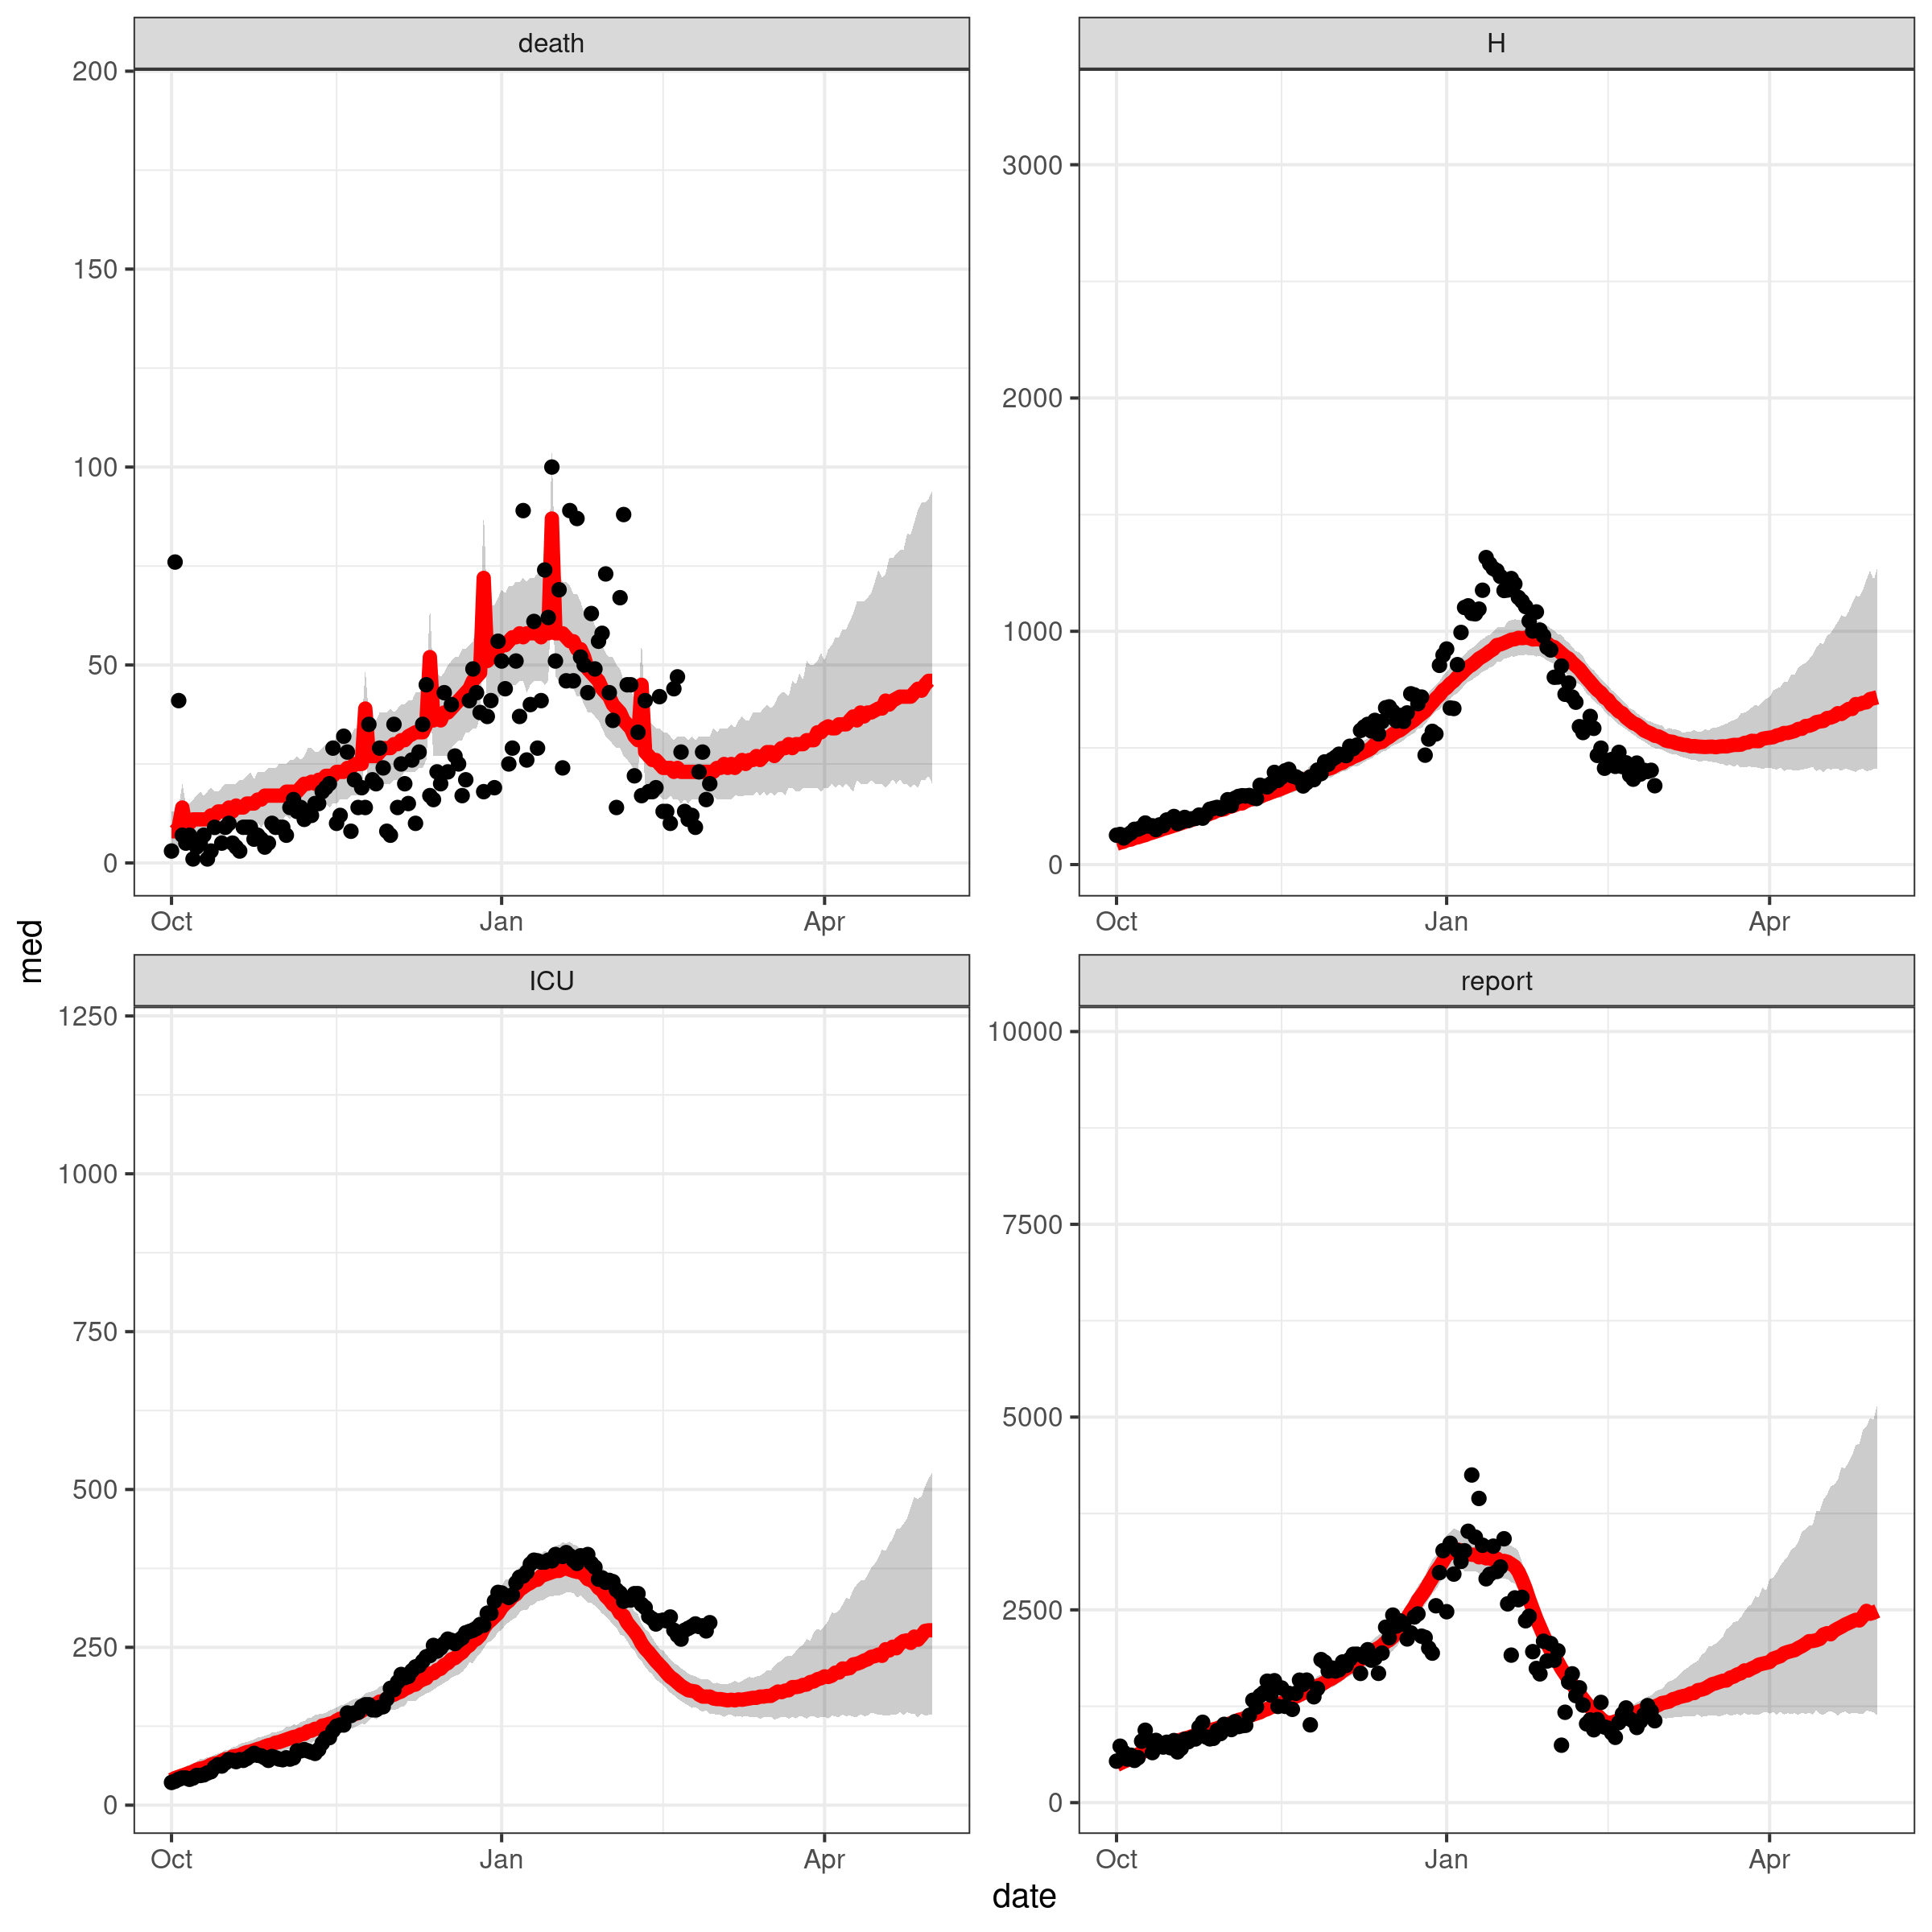
\includegraphics[width=\maxwidth]{code/cachestuff/ontario.png} 

\caption{Ontario calibration}
\label{fig:Ont_calibration}
\end{figure}

\FloatBarrier

\mike{Need to fix hospitalization to fit better. If not maybe get rid of it? Do we want to start from second wave or do the actual fit from March 2020?}

\begin{figure}[ht!]
\definecolor{shadecolor}{rgb}{0.969, 0.969, 0.969}\color{fgcolor}
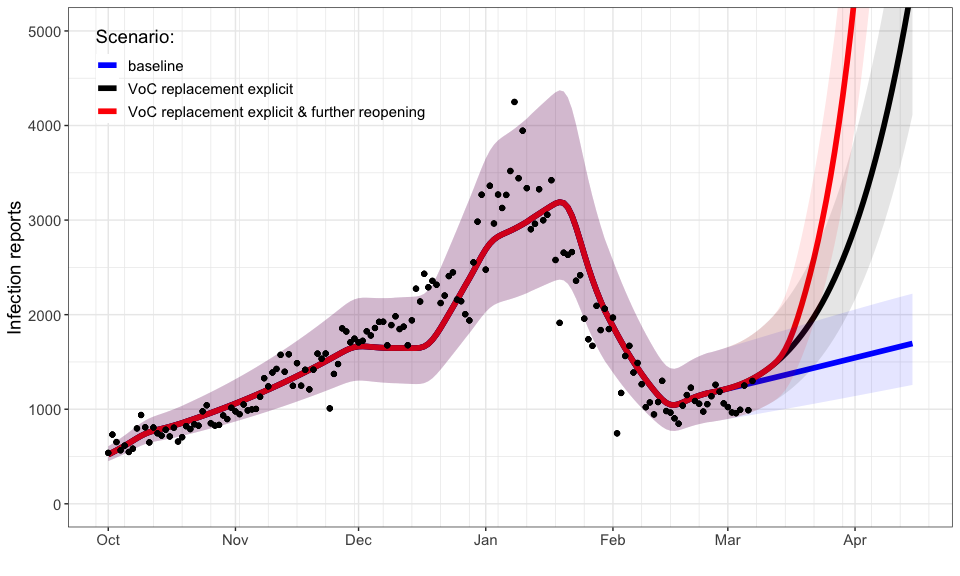
\includegraphics[width=\maxwidth]{code/cachestuff/ontario_voc.png} 

\caption{Ontario calibration}
\label{fig:Ont_voc}
\end{figure}

\FloatBarrier

\mike{Borrowing figure from OMT report. }

\subsection{Limitations}

Our model assumes homogeneous mixing of the population.  No
age-related or spatial contact structure is considered.  In addition,
long-term care facilities (LTCFs), where many elderly people in Canada
have died without going to hospital, have not been modelled
explicitly.  While we do not anticipate any qualitative differences in
results, explicitly creating compartments and calibrating to data for
LTCFs would likely allow us to match ICU occupancy and forecast
pressure on ICUs more accurately.

\subsection{Conclusions}

\mike{conclusion needs to change to match the story}

Testing remains an important surveillance strategy for COVID-19.  In
order to mitigate spread, testing would need to be combined, not only
with isolation of infected individuals, but with extensive contact
tracing and quarantine of contacts.  \david{We need to do more to
  bolster this conclusion, but should be OK for the report.}  More
widespread and faster diagnostic testing \cite{Will+20,Wyll+20} also
have the potential to significantly reduce the spread of SARS-CoV-2.

Future work using our model should focus on estimating how much
testing and tracing is likely to be necessary in order to interrupt
sufficiently many chains of transmission that health care system
burdens remain below tolerable levels.

%%\input{nextsteps.tex}

\clearpage

\section{Appendix: Model calibrations for each province}\label{sec:supp}

Our fits are shown in the \hyperlink{current.fits}{following pages},
with one page per province.  Provinces are ordered by total
population. The smaller provinces (later pages) have far fewer cases
so the fits are less reliable.

The data to which we calibrated the model are shown with dots.
We fitted to hospital occupancy rather than admissions because
we have admissions data only for Ontario.  The fitted model
is shown with solid curves in each panel.
The bottom row shows inferred total disease incidence, 
and 
our mobility index for the province.
\david{[temporarily deleted because we don't have $\R_t$ in the plots]
, and our inferred value of \Rt
(\cref{eq:Rt}). Note that in our current model \Rt\ depends
\emph{only} on the mobility index, the time period (early or late) and
the direct and indirect effects of susceptible depletion.}

\FloatBarrier
\clearpage

%% LOOP THROUGH PROVINCES TO GET FIGURES:
%% Note that we could implement a switch for the captions via:
%%   https://tex.stackexchange.com/questions/64131/implementing-switch-cases

\clearpage

\bibliographystyle{vancouver}
\bibliography{McMasterReport}

\end{document}
